\chapter{Implementation and simulation of QEC codes: Framework setup and baseline models}
\label{chap:implementation_and_simulation}

We have so far conducted a profound theoretical study of the different QEC codes, decoders, and error models. Moving from theory to practice requires specialized computational tools capable of simulating quantum systems efficiently. 

\notatfm{The Gottesman-Knill theorem is referred to in the original Gottesman paper simply as Knill's theorem, as it was initially only privately communicated. It is now commonly known as the Gottesman-Knill theorem to recognize both Knill's original insight and the subsequent formal proof by Gottesman using his Stabilizer formalism.}
Simulating arbitrary quantum circuits is exponentially hard for classical computers; however, the Gottesman-Knill theorem \cite{gottesman1998heisenberg} guarantees that circuits restricted to Clifford group operations (which include stabilizer measurements, CNOTs, and Pauli gates) can be simulated efficiently in polynomial time. 

In this chapter, we establish our experimental framework using \texttt{stim} \cite{gidney2021stim}, a high-performance Clifford simulator that relies on the referred Gottesman-Knill theorem and its subsequent improvements by Aaronson and Gottesman\cite{aaronson2004improved}, and incorporates some additional improvements. We will build our simulations progressively: starting with a basic repetition code to understand the mechanics of syndrome extraction and decoding, moving through different noise models, and finally implementing the 9-qubit Shor code to empirically demonstrate the Threshold Theorem.

\section{Simulating QEC codes and decoders with \texttt{stim}}
\label{sec:simulating_with_stim}

Stim is a QEC specialized simulator. The primary advantage of \texttt{stim} is its ability to sample detection events --syndromes-- and logical observables --flips in the logical state of our code-- extremely fast. Instead of tracking the full state vector, it tracks how Pauli errors propagate through the circuit. To utilize this tool, a QEC simulation requires three main components: a circuit defining the code structure, a noise model that injects errors, and a classical decoder that interprets the syndromes.

\subsection{Simulating the repetition code under code-capacity noise}
\label{subsec:repetition_code_sim}

To introduce the simulation pipeline, we begin with the simplest QEC protocol: the distance-$d$ repetition code. As discussed in Chapter \ref{chap:introduction}, this code protects against a single type of error (e.g., bit-flips) by encoding one logical qubit into $d$ physical data qubits, requiring $d-1$ additional ancilla qubits to perform parity measurements.

For our baseline simulation, we use a \textbf{code-capacity noise model}. For our baseline simulation, we use a code-capacity noise model (see Chapter \ref{chap:modeling_quantum_error}) using a depolarizing channel. 

Stim makes it exceptionally easy to implement a basic repetition code. The building blocks of this simulation are:
\begin{itemize}
    \item \textbf{The QEC code circuit}. \texttt{stim}'s library already provides a method to easily generate a basic repetition code. This generates not only the circuit for the encoding, but the necessary ancilla qubits and measurements for syndrome extraction.
    \item \textbf{Injecting the error}. As part of building the circuit, \texttt{stim} allows inputing the physical error rates for different types of noise. In this case, to simulate code-capacity noise, we use the parameter \verb|before_round_data_depolarization|.
    \item \textbf{Decoding the error}. The \texttt{pymatching} library will allow us to decode the error using the MWPM algorithm that we discussed in Chapter \ref{chap:qec_decoders}. For such decoding to happen, \texttt{stim} requires the circuit to have specific tags appended (\texttt{DETECTORS}) to specific measures. In this example, the generated circuit already contains them.
\end{itemize}

The code in Listing \ref{lst:stim_rep_code} illustrates how this simulation can be performed. It is important to understand how \texttt{stim} works.  The \texttt{sample} method returns two things:

\begin{enumerate}
    \item A binary array of detection events (in the code, \texttt{syndromes}). It contains one value for each measured detector. The value is $0$ if the detector observed the expected parity, and $1$ if the detector was activated, indicating the presence of an error.
    \item A binary array of logical outcomes (in the code, \texttt{actual\_observables}). Rather than representing logical states, these values act as boolean flags. A value of $1$ indicates that the accumulated physical errors during that shot successfully flipped the corresponding logical observable.
\end{enumerate}

\notatfm{The preparation of the initial state of a circuit is not generally required. However, noise models can be asymmetric (e.g. a qubit may be more likely to flip from $\ket{1}$ to $\ket{0}$ than from $\ket{0}$ to $\ket{1}$) and so can be QEC codes (the 9-qubit Shor code has better protection against bit-flip errors than against phase-flip errors). In these cases, preparing the initial state may be required.}
During the simulation, errors can occur with a certain probability $p$. When they happen, they are tracked and cascade down to the detectors and observables, allowing \texttt{stim} to determine both if a detector is triggered and if an observable flips. If the code and the decoding succeed, both should match. Because flips, rather than states, are tracked, the circuit does not have to be prepared on a certain state, we only evaluate its capacity to preserve its state.

Figure \ref{fig:stim_rep_compare_plot} shows the logical error rate as a function of the physical error rate for this code with two different decoders. Note that, as a basic repetition code, this code only corrects for bit-flip errors.


\includesnippet[caption={Simulation 1: Basic repetition code simulation}, label={lst:stim_rep_code}]{S1_SNIPPET}{../src/chapter_5/s1_stim_rep_code.py}


\subsection{Decoders: From Minimum Weight Perfect Matching to Custom Logic}
\label{subsec:decoders_intro}

Once the circuit is executed and noise is applied, \texttt{stim} outputs an array of detection events. The role of the decoder is to map these events to a predicted logical error. 

As seen in Chapter \ref{chap:qec_decoders}, the standard approach for 1D repetition codes and 2D surface codes is the \textbf{Minimum Weight Perfect Matching (MWPM)} algorithm. In our framework, we implement this using the \texttt{PyMatching} library.

To better understand the internal workings of a decoder, we implement a custom \textbf{Majority Vote Decoder}. Unlike the graph-based approach of MWPM, this decoder resolves errors by directly evaluating the local parity checks and "voting" on the most likely state of the data qubits. 

\notatfm{Note that we show here the specific part of the code that decodes a single shot of the sampling. When the circuit is simulated,  multiple shots are run to get statistically significant information}
The code Listing \ref{lst:majority_vote_decoder} shows a very simple implementation of such decoder, which can be used with the same repetition circuit created in Listing \ref{lst:stim_rep_code}. 

\includesnippet[caption={Simulation 2: Implementation of a simple Majority Vote decoder for a repetition code}, label={lst:majority_vote_decoder}]{S2_SNIPPET}{../src/chapter_5/s2_majority_vote_decoder.py}

As seen in Figure \ref{fig:stim_rep_compare_plot}, for simple repetition codes under basic noise models, both decoders perform similarly, effectively reducing physical errors. In the following section we will stress-test our decoders to see how their efficiency decays with different noise models.

\begin{figure}[hbt!]
    \centering
    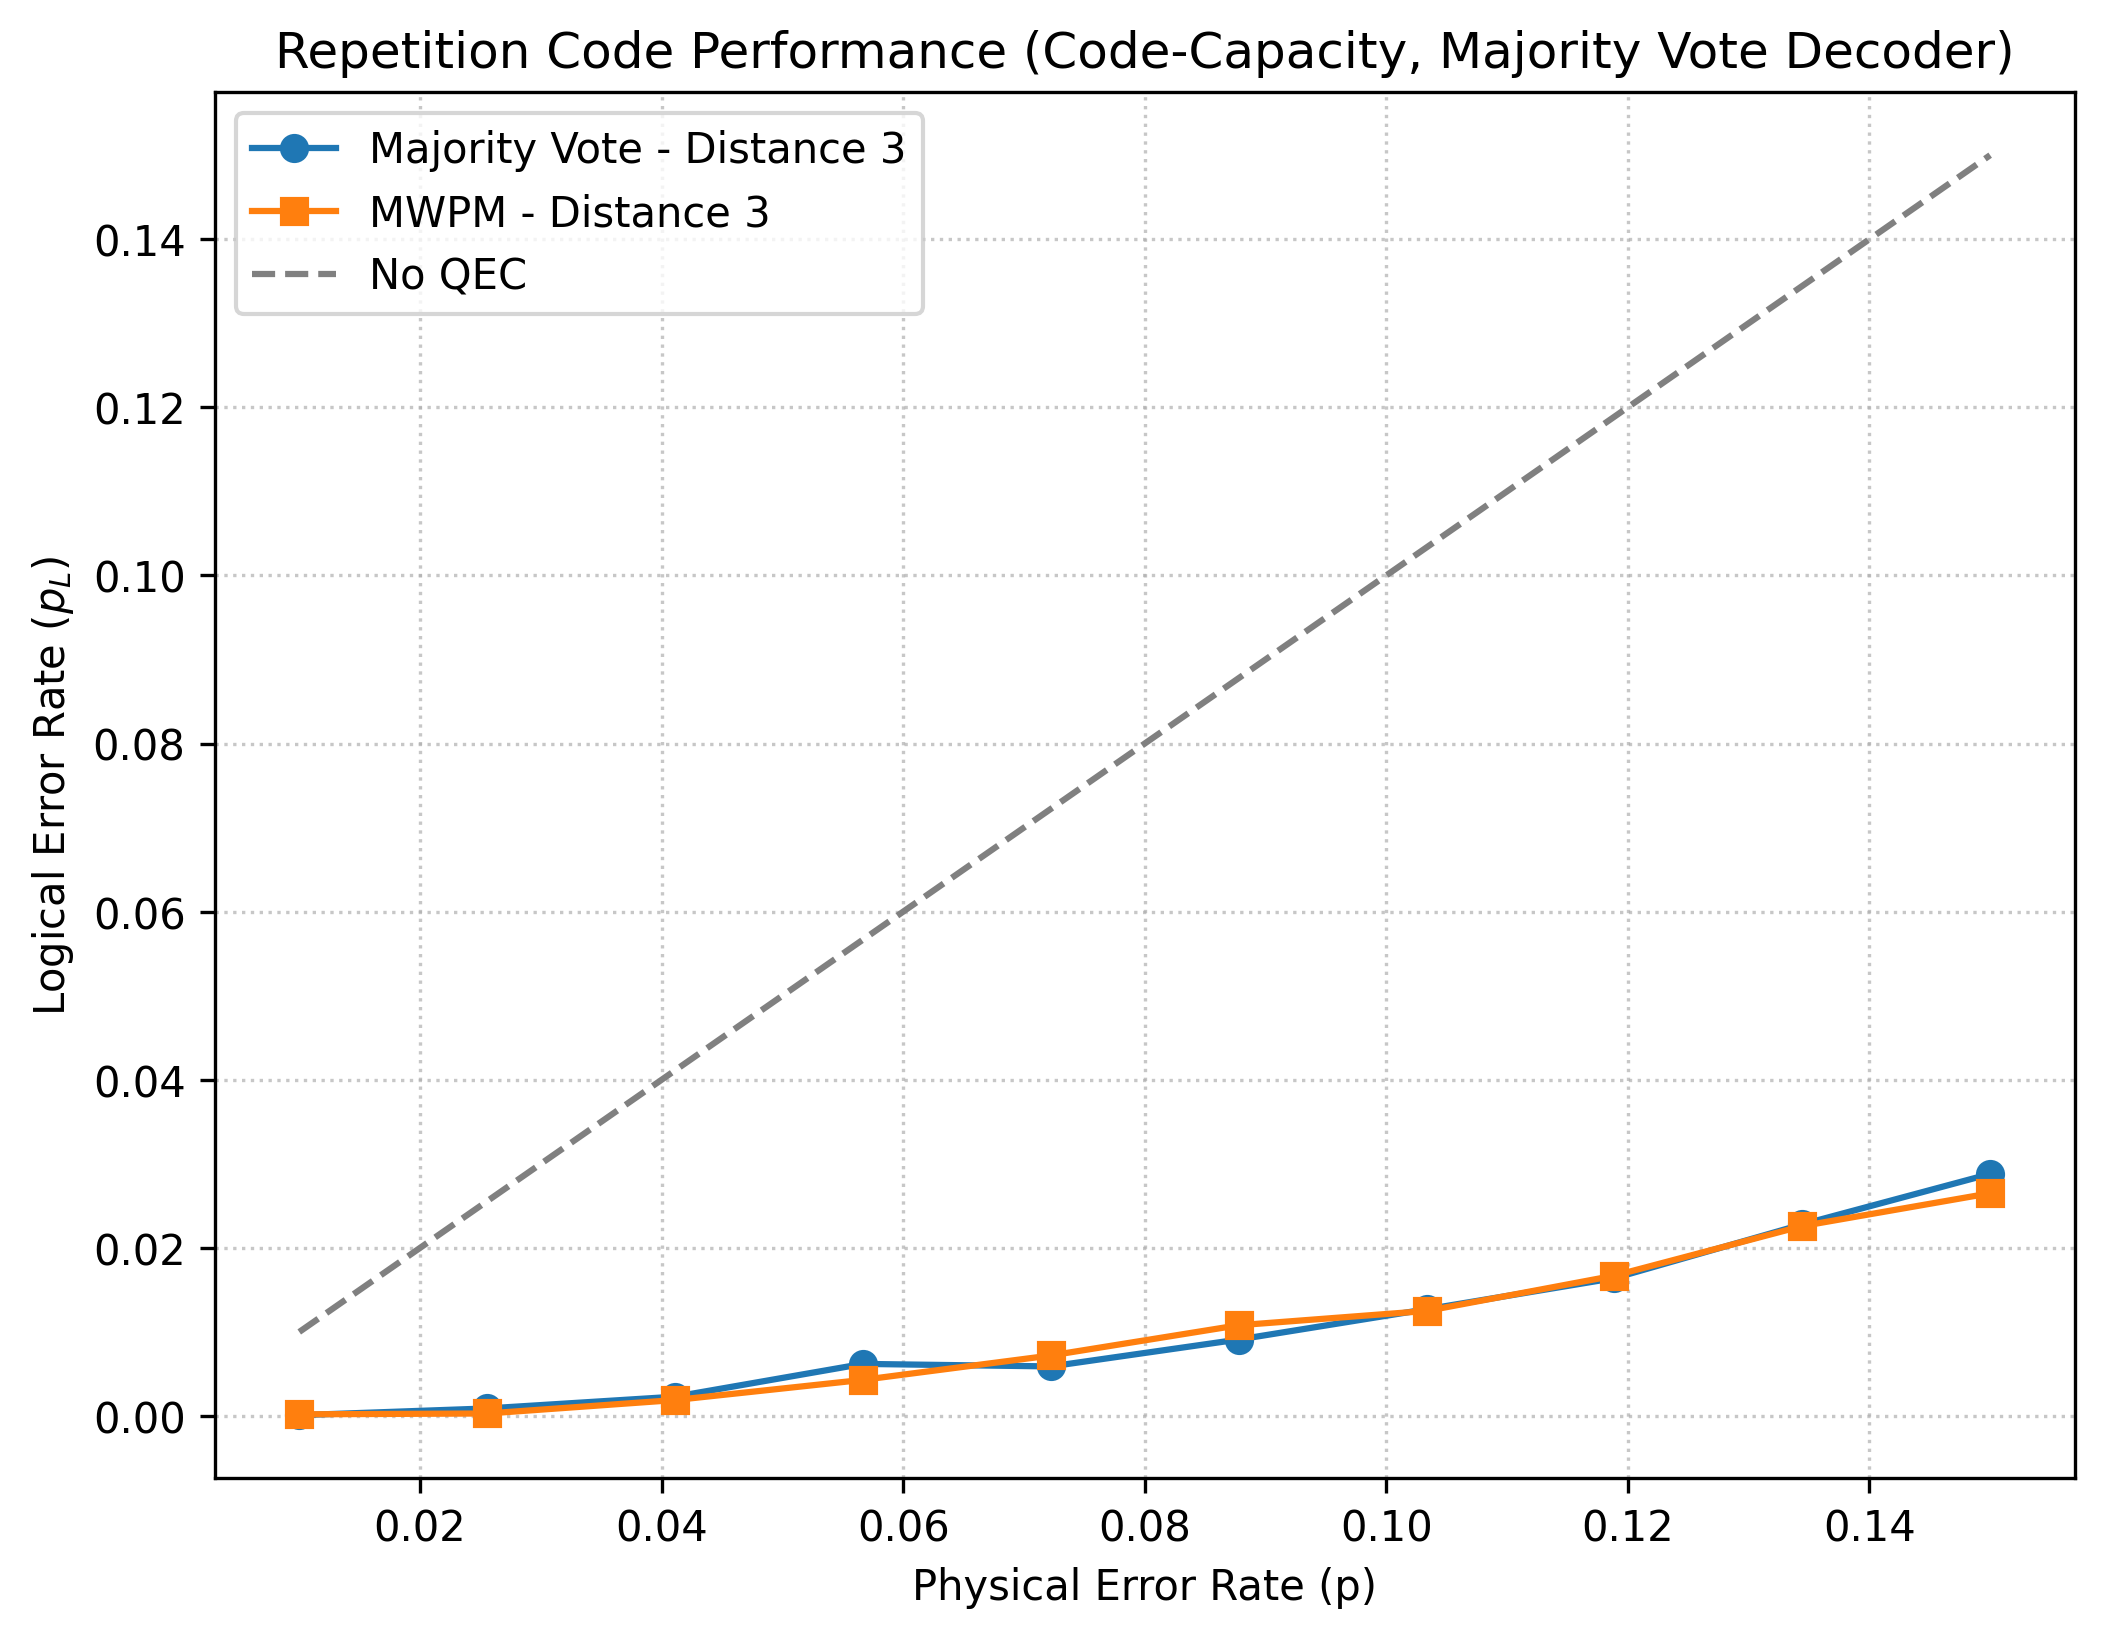
\includegraphics[width=0.6\linewidth]{figures/stim_rep_comparison_plot.png}
    \caption{Simulation 3: Comparison of the results of simulations 1 and 2. Displays the logical error for a basic repetition code using Majority Vote and MWPM decoders. The x=y dotted line helps comparing the QEC protocol to not implementing any QEC. If the logical error rate is above the physical error rate, the QEC protocol is adding errors}
    \label{fig:stim_rep_compare_plot}
\end{figure}

\subsection{Introducing circuit-level noise}
\label{subsec:circuit_level_noise}

While the code-capacity model is useful for validating decoders, it does not reflect physical reality. In a real quantum computer, the gates used to entangle the qubits and the measurements used to extract the syndrome are themselves noisy.

To illustrate this, we expand our simulation to include \textbf{circuit-level noise}. As seen in Chapter \ref{chap:modeling_quantum_error}, in this model, we inject depolarizing noise into single-qubit and two-qubit gates, and we add a probability of measurement readout errors. For the purpose of this test, we will use a very simple noise model, where the three types of noise added to the circuit have the same probability (ratio 1:1:1). This is easily implemented with \texttt{stim} in the circuit creation, as seen in Listing \ref{lst:stim_rep_code_noise}.

\includesnippet[caption={Simulation 4: Adding circuit-level noise.}, label={lst:stim_rep_code_noise}]{S4_SAMPLE}{../src/chapter_5/s4_majority_vote_noise.py}

As shown in Figure \ref{fig:stim_rep_circuit_distance_plot}, realistic noise drastically reduces the effectiveness of the code, but it also shows the importance of the decoder. Handling circuit-level noise requires complex spatial-temporal decoding graphs, which makes MWPM a better solution than a basic Majority Vote decoder. The figure also shows how increasing the distance improves the results of the MWPM decoder, but it degrades the result of the Majority Vote decoder. This means that, for this specific noise model and the MWPM decoder, the system is operating under the threshold, so the error correcting capacity of the protocol can be increased by increasing the distance. However, with our Majority Vote decoder, the system operates above the threshold.

\begin{figure}[hbt!]
    \centering
    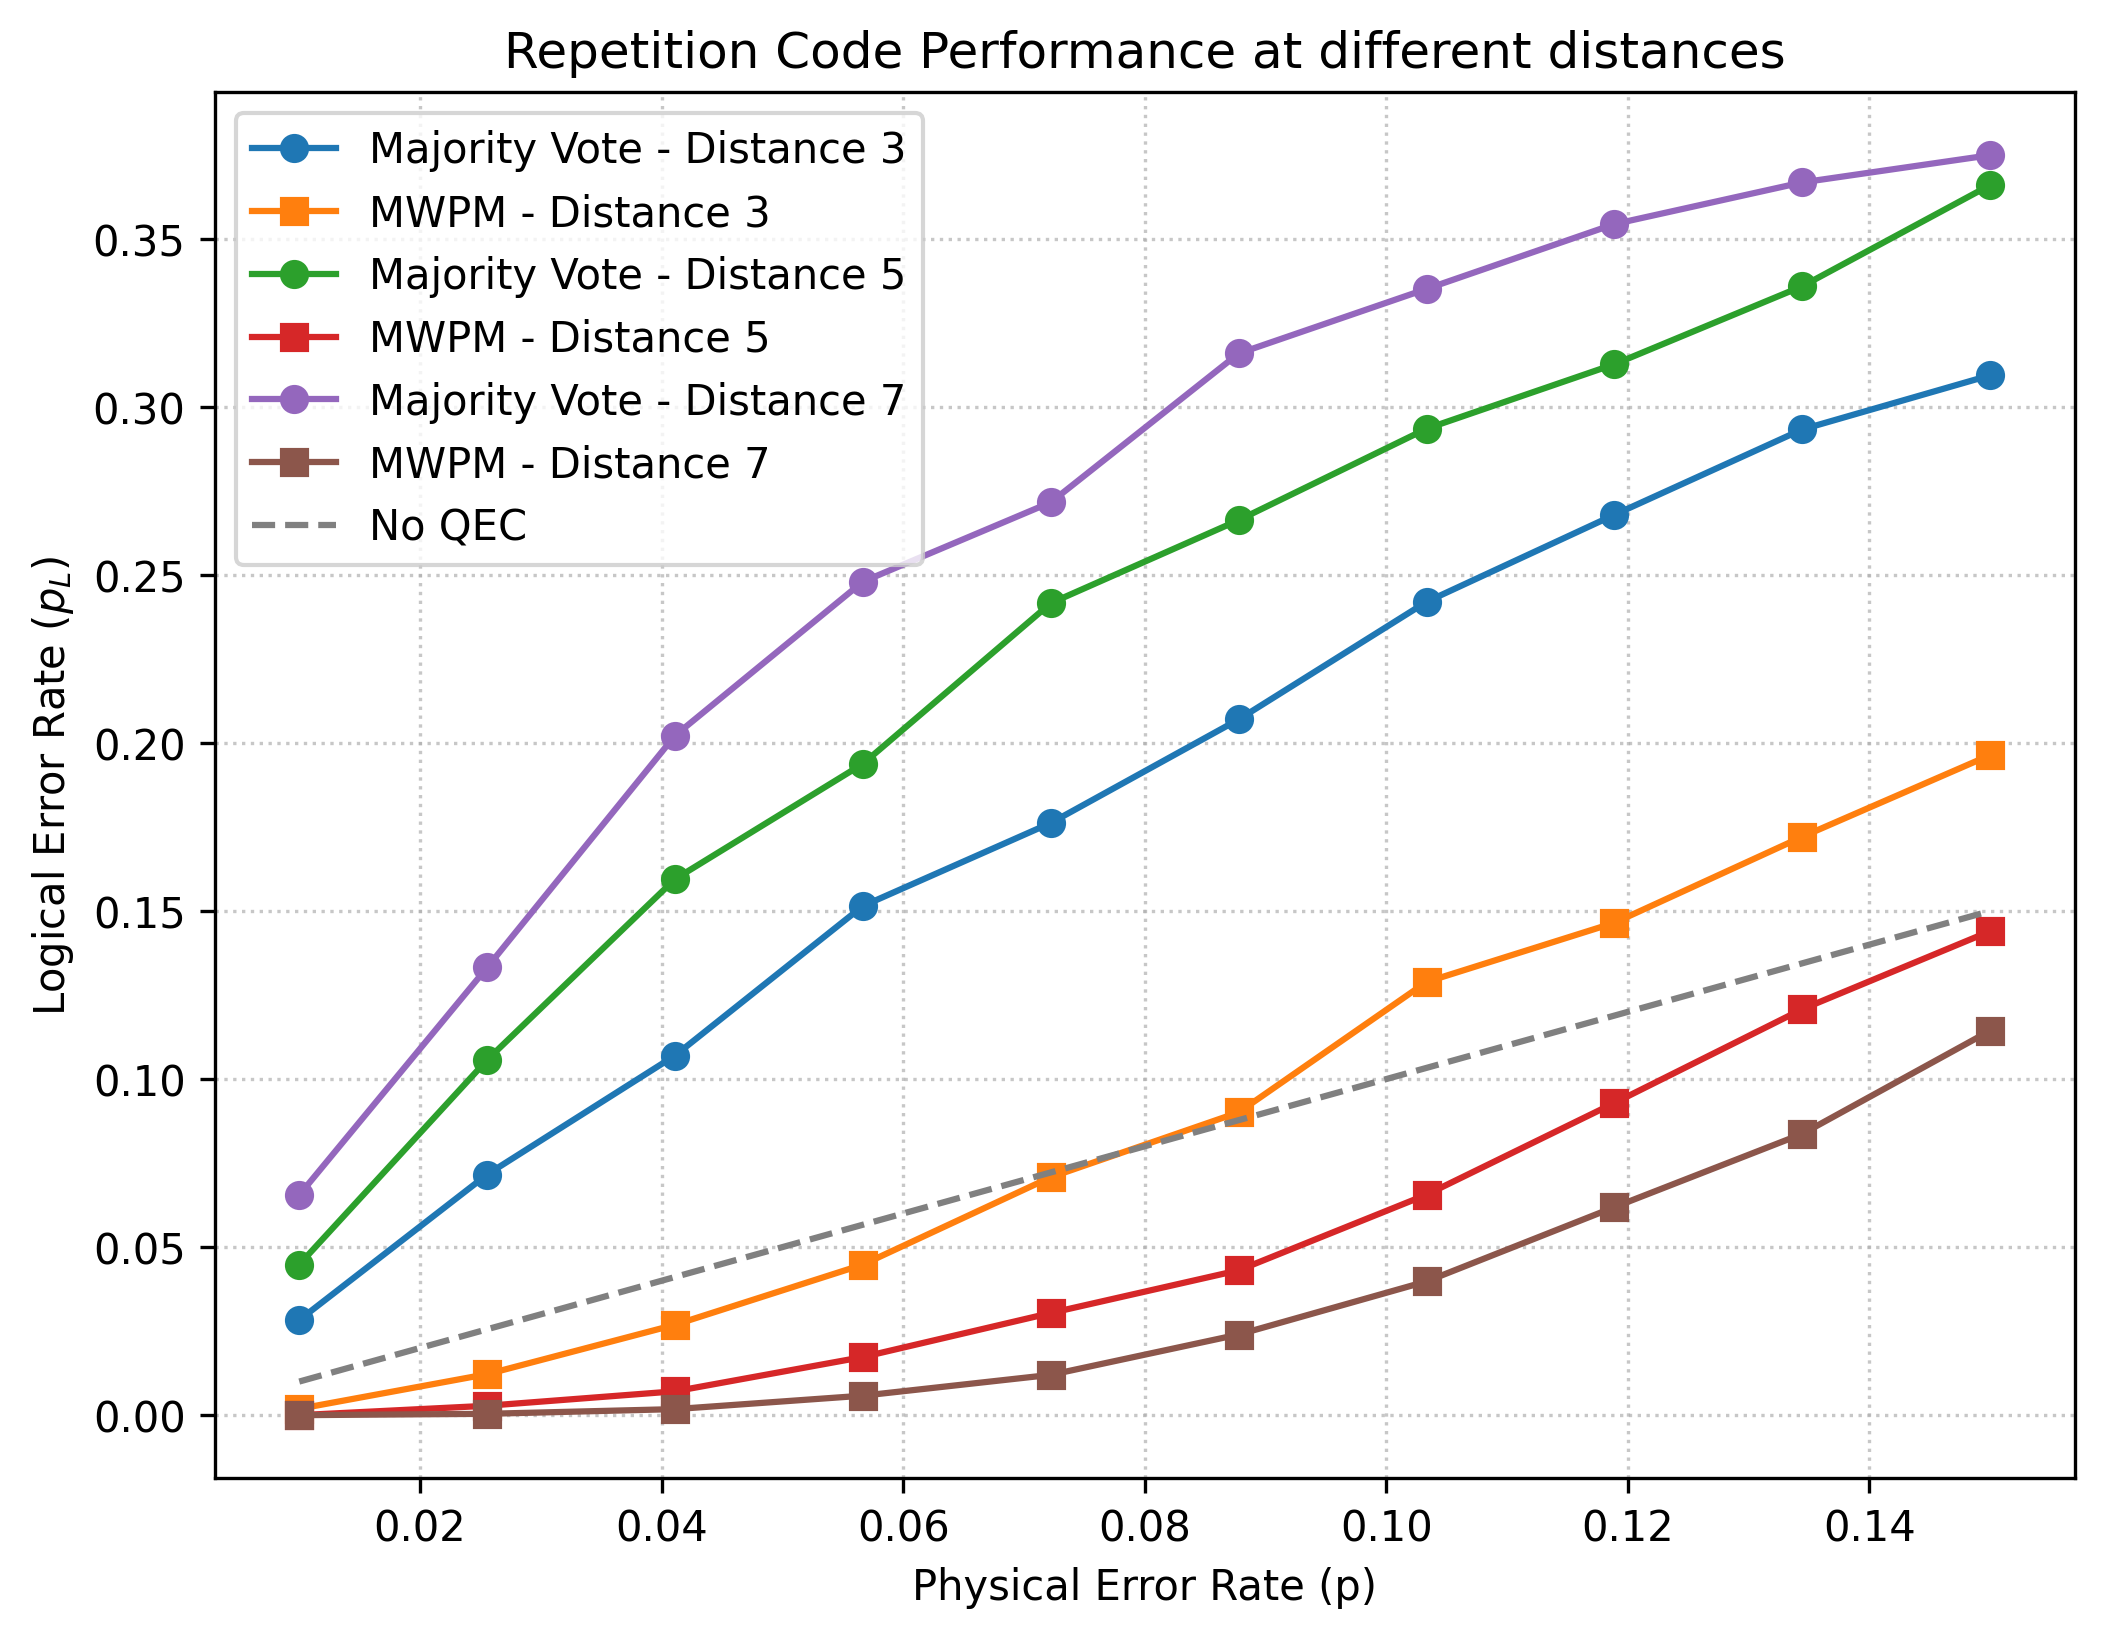
\includegraphics[width=0.8\textwidth]{figures/stim_rep_circuit_distance_plot.png}
    \caption{\textbf{Simulation 4}: Impact of circuit-level and phenomenological noise on the repetition code performance. Introducing more complex noise significantly degrades the logical error suppression compared to the idealized code-capacity baseline. With this additional noise, MWPM shows its advantage over the Majority Vote because of its capacity to consider the probabilities of each error to select the most probable set of errors that could have caused the observed syndrome. 
    \textbf{Simulation 5}: Under a complex noise model (code-capacity, circuit-level and phenomenological) increasing the distance of the code has the opposite effect for each of the decoders.}
    \label{fig:stim_rep_circuit_distance_plot}
\end{figure}

\begin{figure}[hbt!]
      \centering
      \begin{subfigure}[b]{0.48\textwidth}
          \centering
          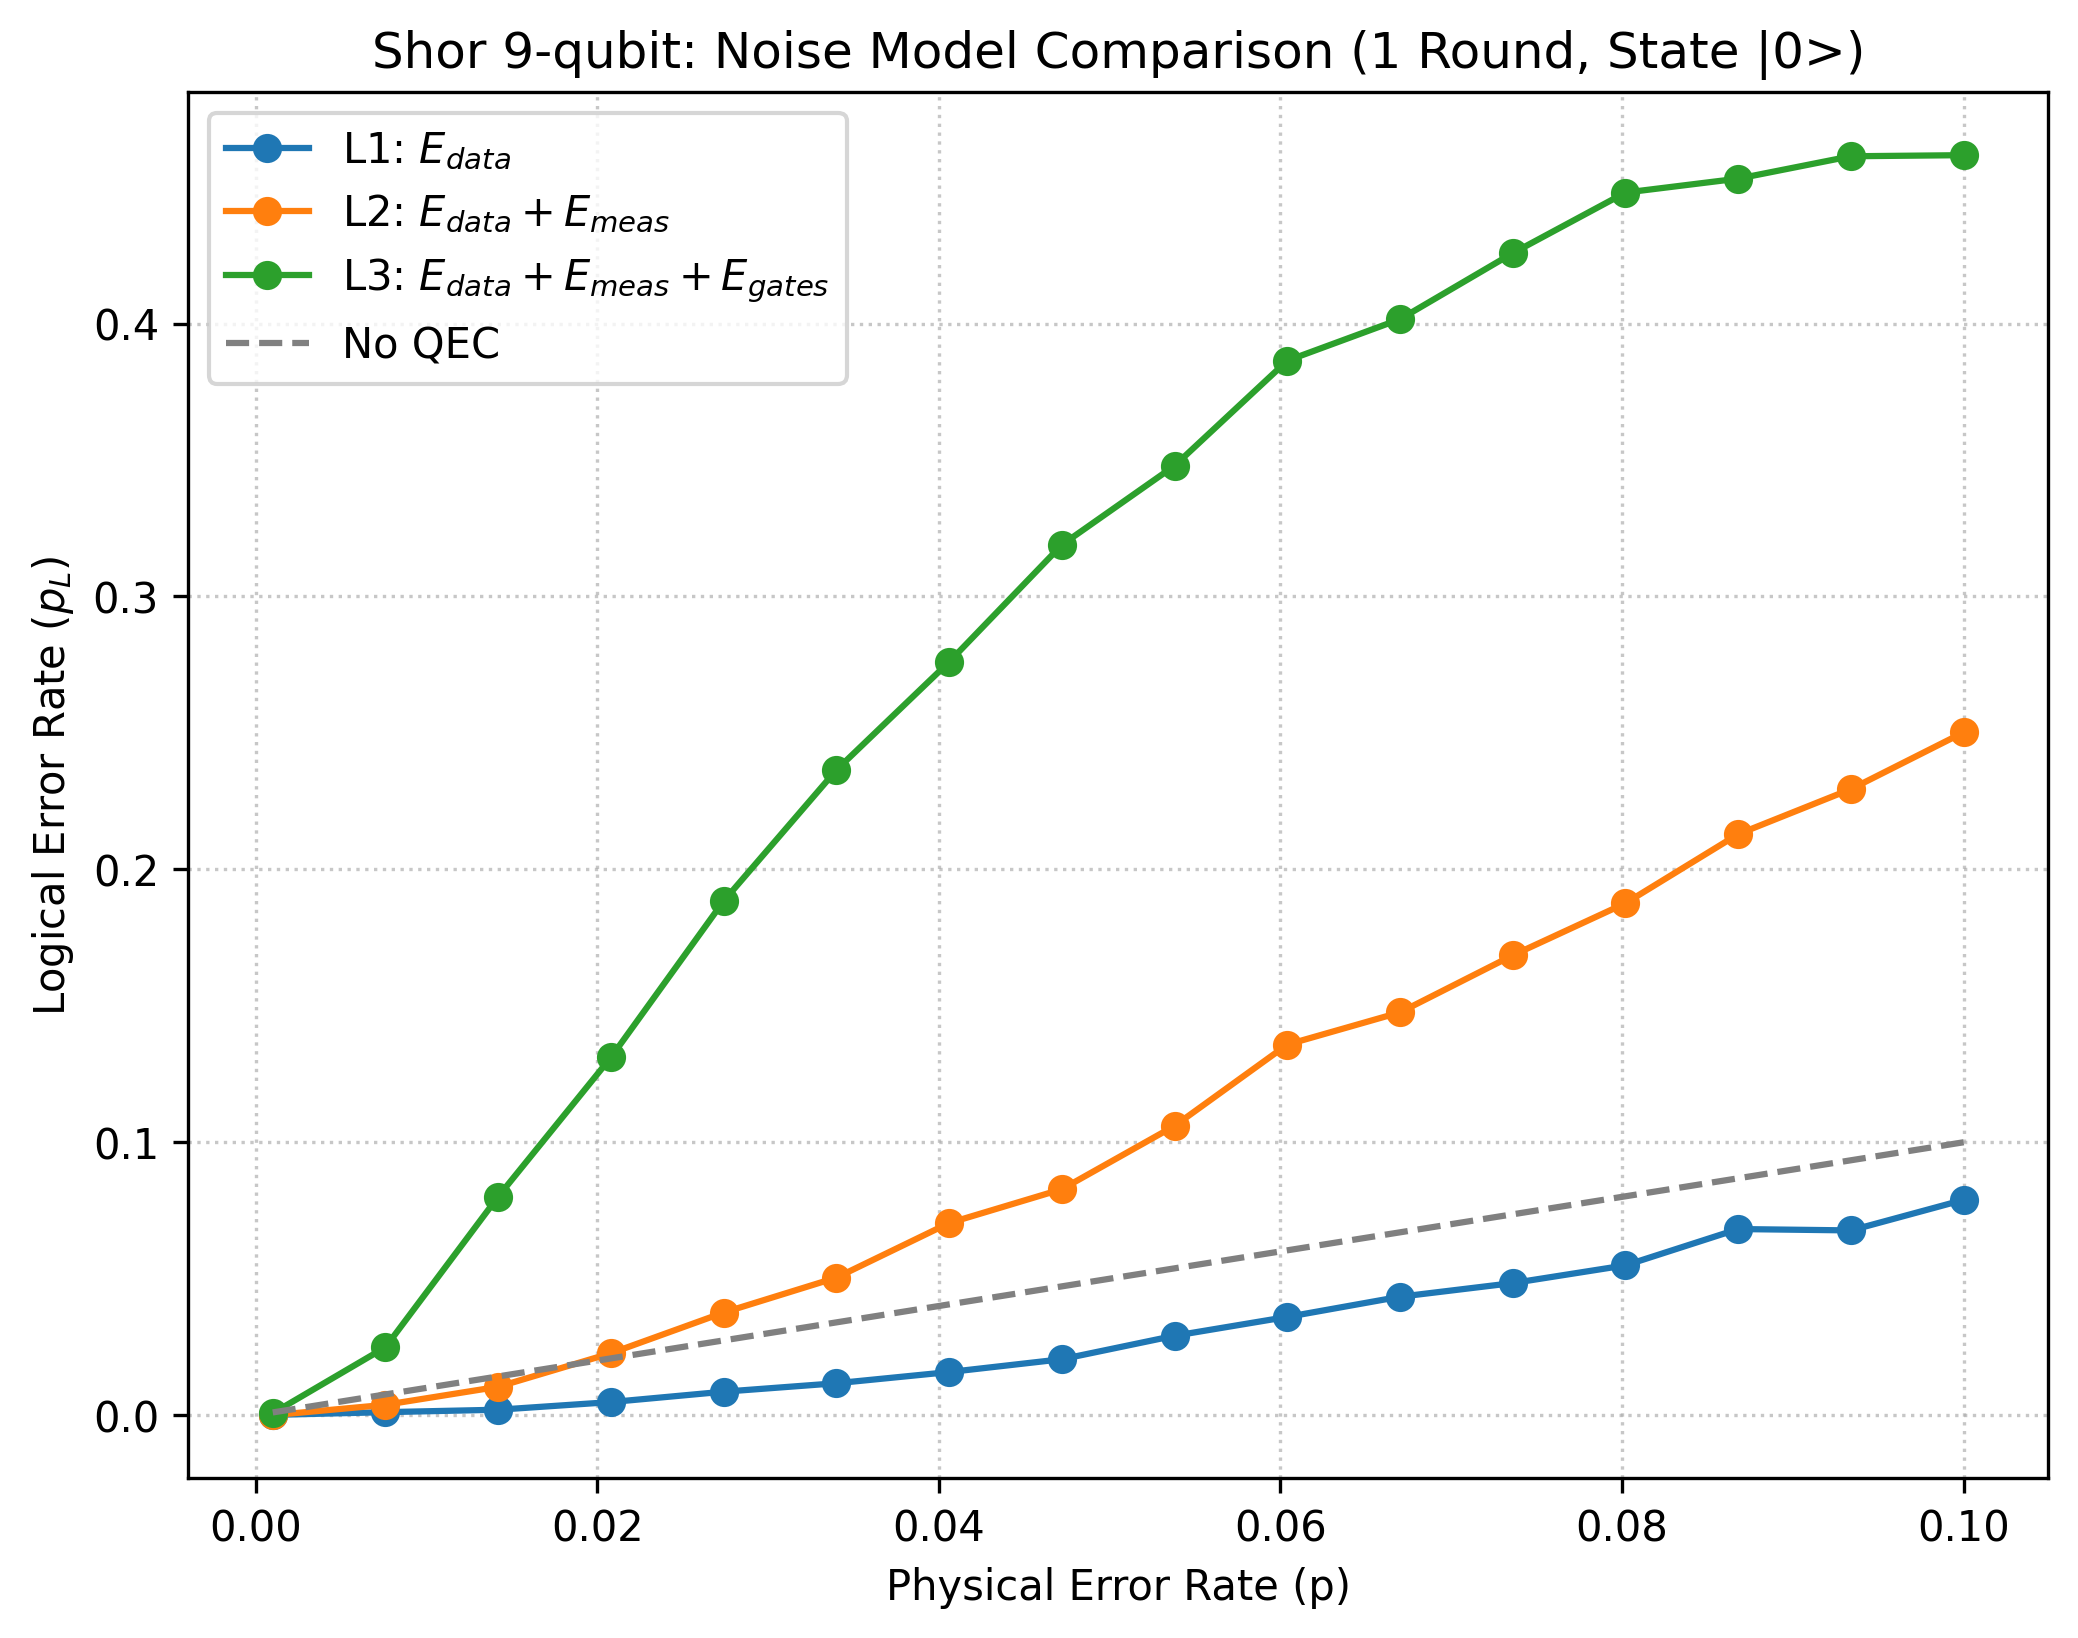
\includegraphics[width=\textwidth]{figures/shor_9_noise_models.png}
          \caption{Noise Model Comparison}
          \label{fig:shor_9_noise_models}
      \end{subfigure}
      \hfill
      \begin{subfigure}[b]{0.48\textwidth}
          \centering
          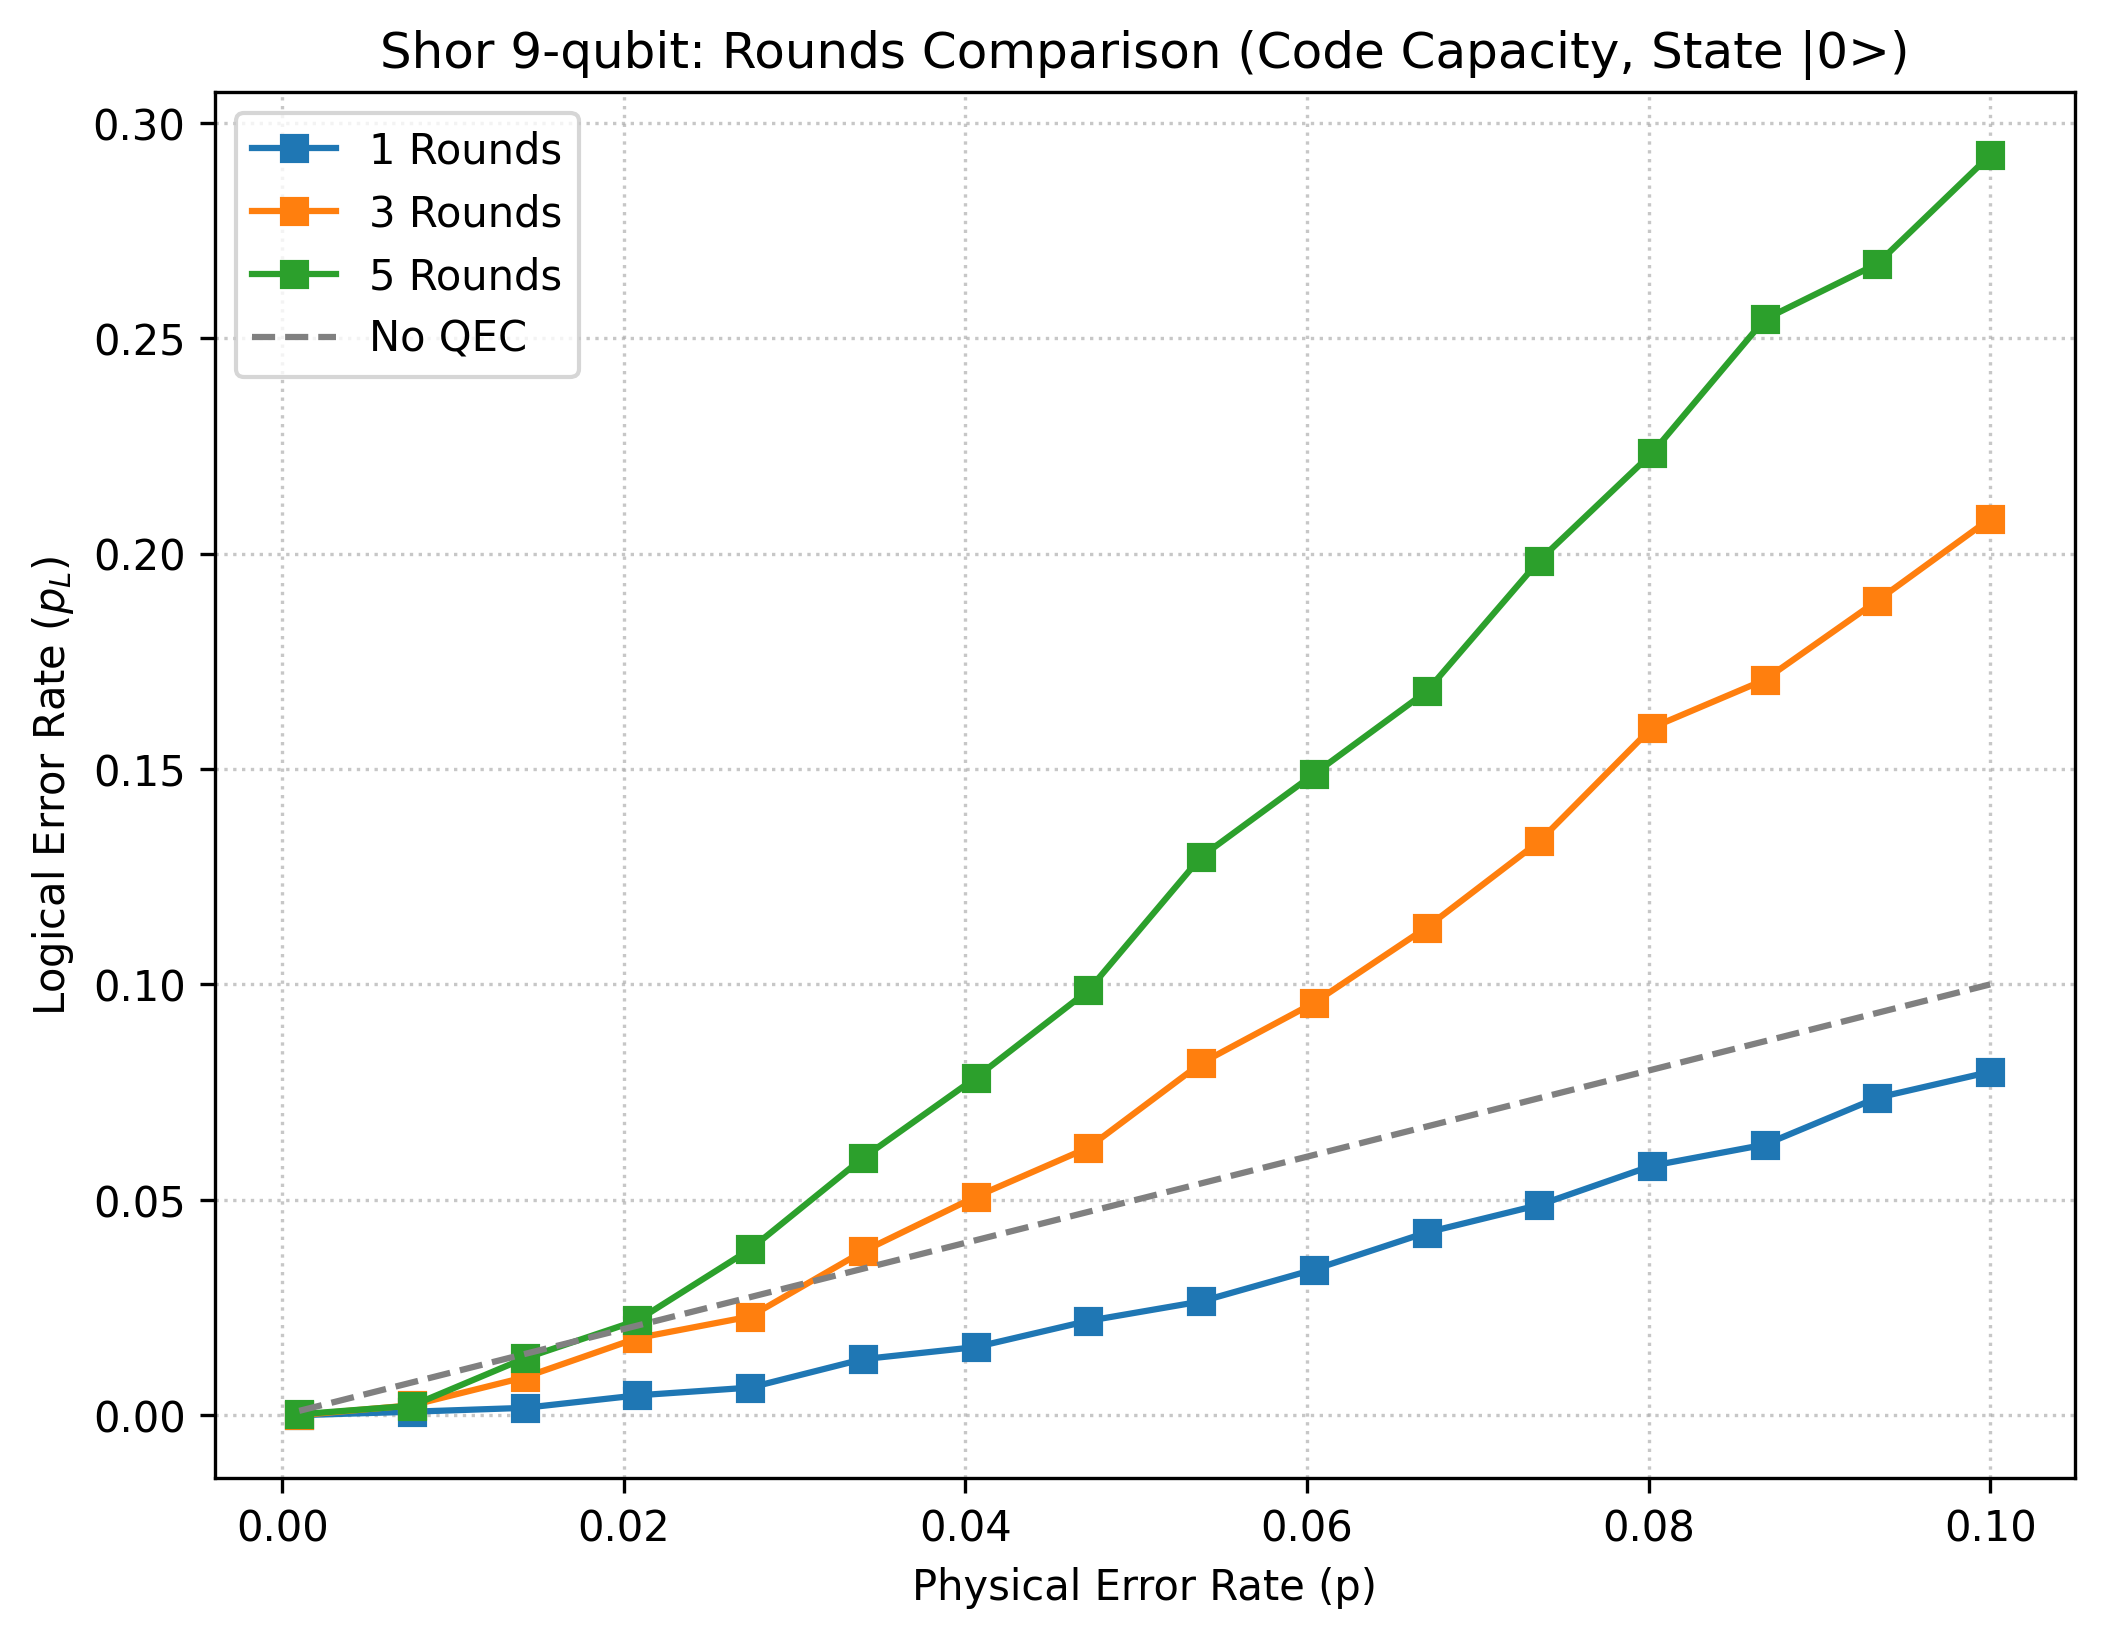
\includegraphics[width=\textwidth]{figures/shor_9_rounds.png}
          \caption{Rounds Comparison}
          \label{fig:shor_9_rounds}
      \end{subfigure}
      \vskip\baselineskip
      \begin{subfigure}[b]{0.6\textwidth}
          \centering
          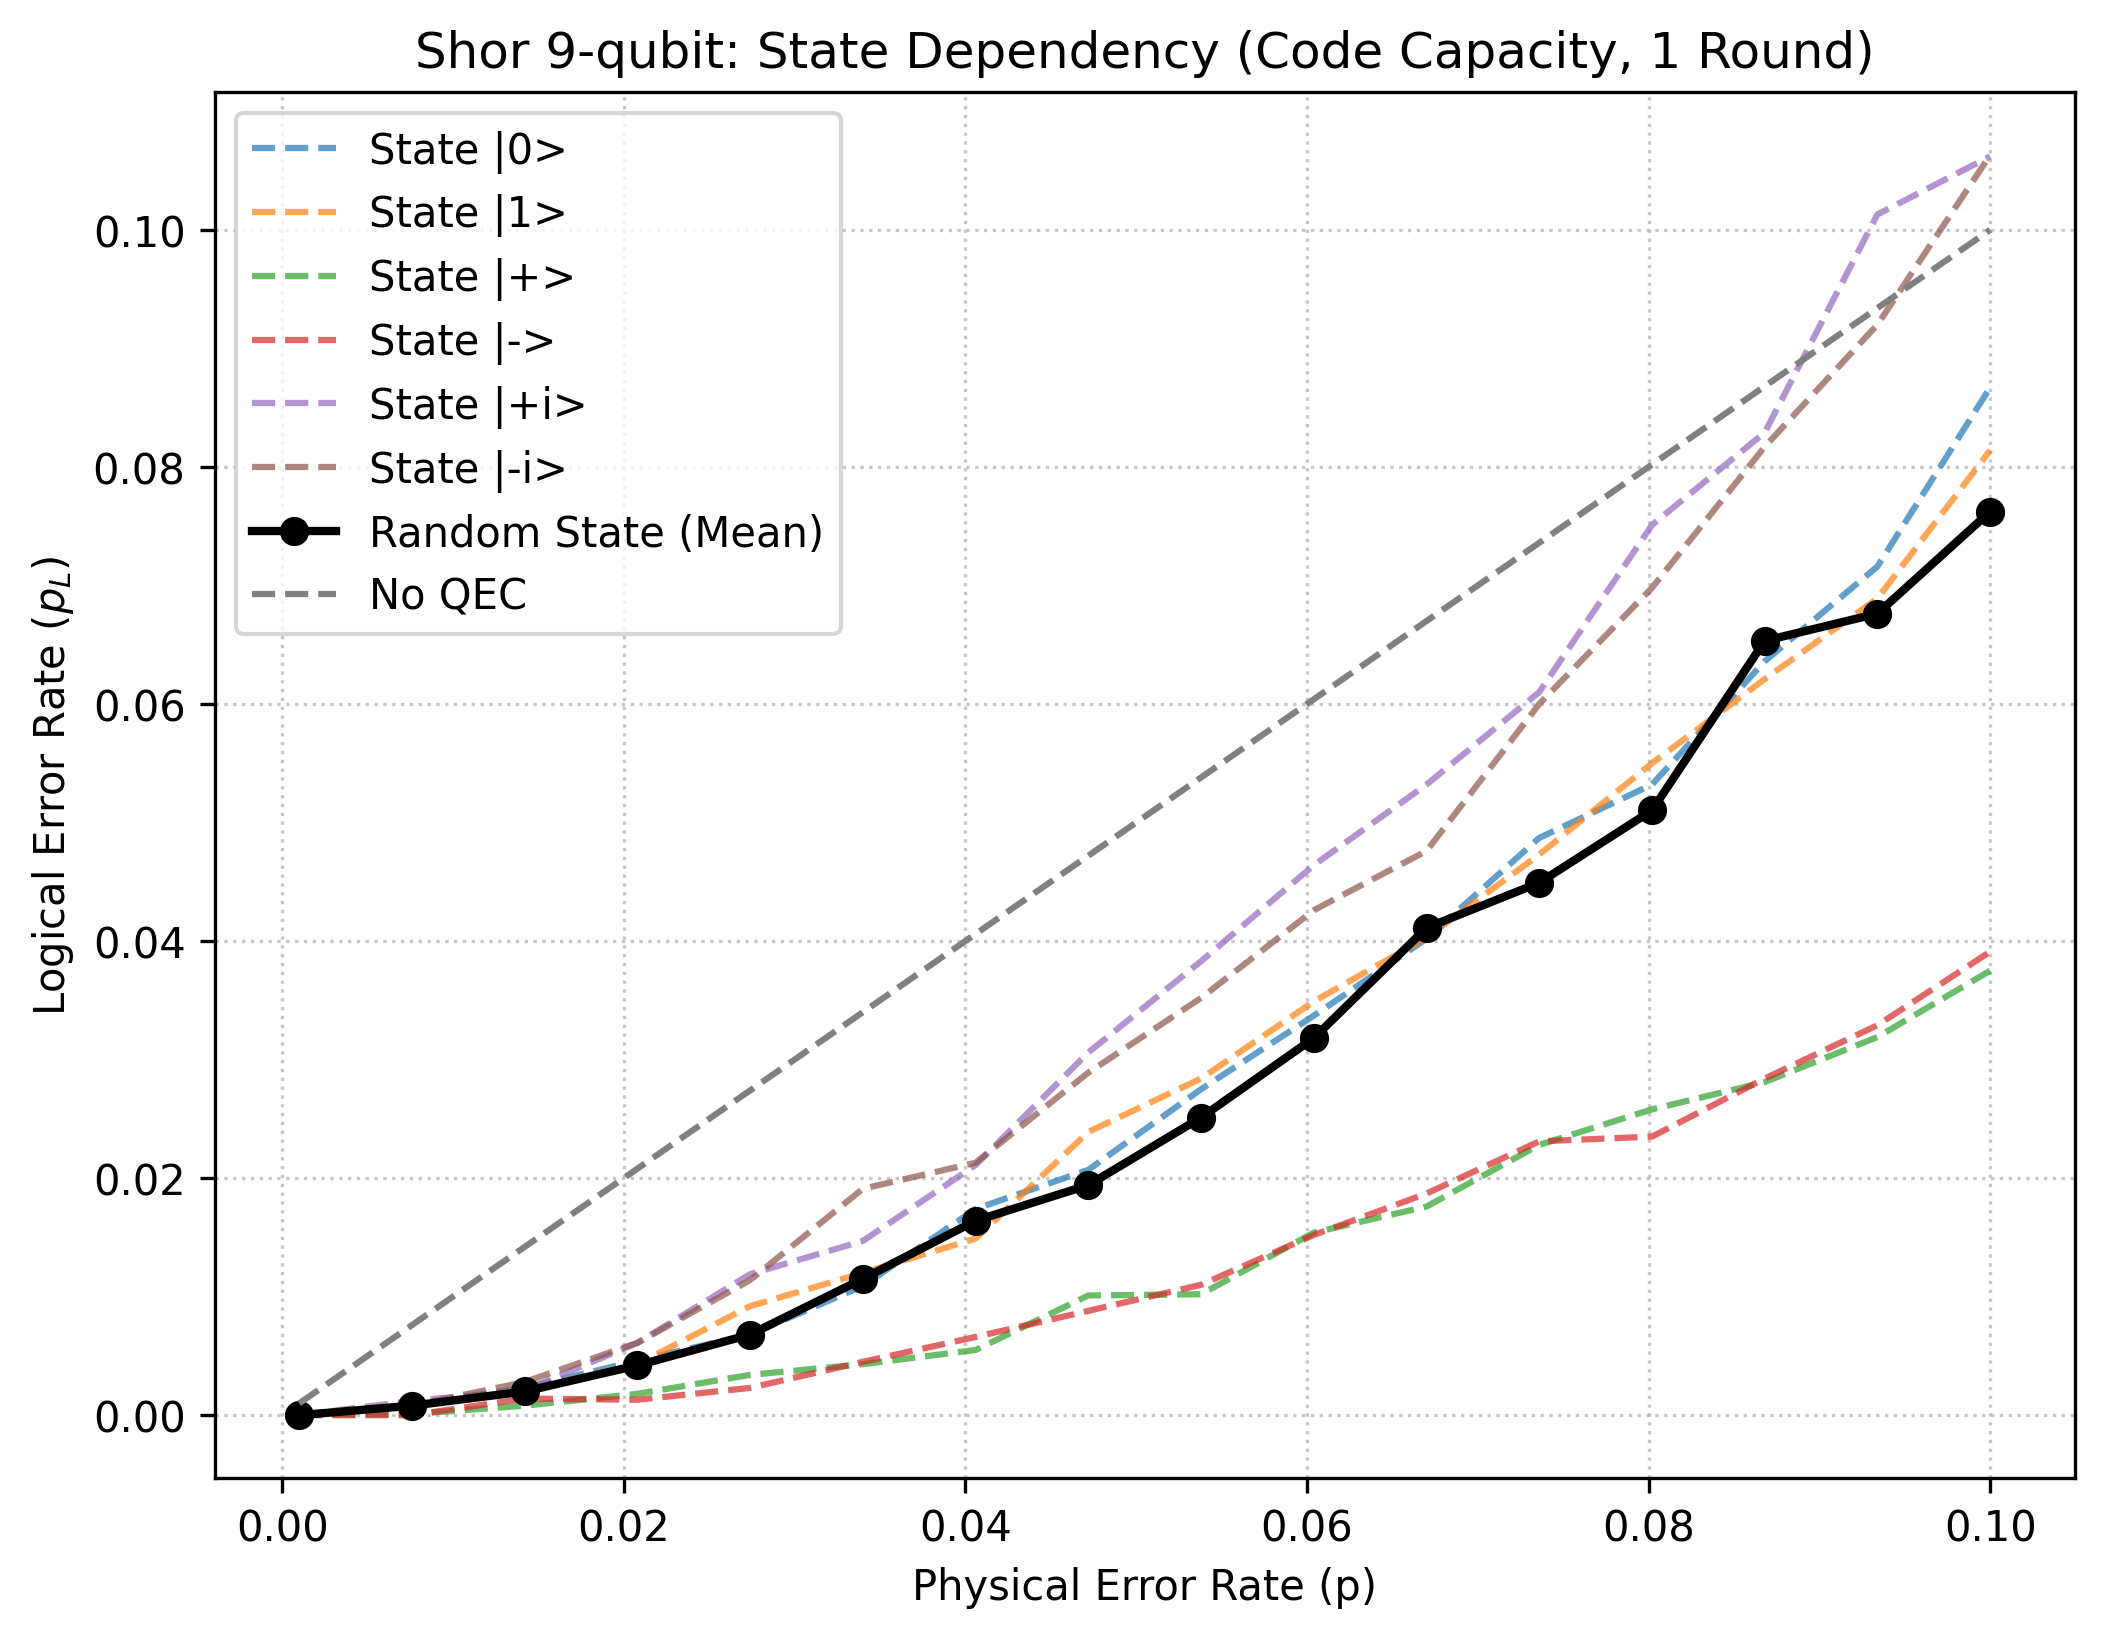
\includegraphics[width=\textwidth]{figures/shor_9_states.png}
          \caption{State Dependency}
          \label{fig:shor_9_states}
      \end{subfigure}
      \caption{\textbf{Simulation 6}: Performance analysis of the Shor 9-qubit code using the MWPM decoder. 
      \textbf{(a) Comparison of noise models}: Three levels of noise complexity are evaluated: 1) \textit{Code-capacity}, where noise is only applied to data
  qubits while gates and measurements remain ideal; 2) \textit{Phenomenological}, which adds bit-flip errors to the measurement outcomes; and 3)
  \textit{Circuit-level} (or Circuit-capacity), the most realistic model where depolarizing noise is applied after every Clifford gate and bit-flip noise is
  applied to every measurement. The results show that circuit-level noise significantly increases the logical error rate ($p_L$).
      \textbf{(b) Rounds Comparison}: Evaluates the accumulation of errors as the number of syndrome measurement rounds increases. 
      \textbf{(c) State Dependency}: Shows the performance for different cardinal states ($|0\rangle, |1\rangle, |+\rangle, |-\rangle, |+i\rangle,
  |-i\rangle$). The Shor code provides protection by concatenating a 3-qubit bit-flip code (inner) with a 3-qubit phase-flip code (outer). This structure
  allows the code to correct a single bit-flip ($X$) within each of the three 3-qubit blocks and a single phase-flip ($Z$) across the three blocks. This
  hierarchical protection leads to slight variations in $p_L$ depending on whether the state is more sensitive to $X$ or $Z$ noise components.}
      \label{fig:simulation_6_shor}
  \end{figure}

\subsection{Implementing the 9-qubit Shor code}
\label{subsec:shor_implementation}

\notatfm{Because the final measurement of the data qubits can also be noisy, we must add one last set of detectors at the end of the circuit. These detectors, known as boundary detectors, compare the parity of the final data measurements against the last syndrome extracted via ancillas, effectively catching readout errors in the final layer.}
In our previous simulations, we relied on \texttt{stim}'s built-in circuit generation library. To better illustrate how a quantum error correction circuit is explicitly constructed from scratch, we now implement the 9-qubit Shor code ($[[9, 1, 3]]$). Building a custom circuit in \texttt{stim} follows a strict pipeline.

First, the circuit is declared and initialized, followed by the application of the necessary gates to encode the logical state and extract the stabilizer operators. A crucial step in custom \texttt{stim} circuits is explicitly tracking the outcomes: stabilizer measurements must be labeled as \texttt{DETECTOR}s (Listing \ref{lst:stim_detector}), while the final measurements of the data qubits are targeted by \texttt{OBSERVABLE\_INCLUDE} instructions to track the logical state parity (Listing \ref{lst:stim_boundary_detector_and_observable}). This strict labeling allows the simulator to decouple the syndrome extraction—which provides the inputs for the decoder—from the logical observable tracking, which is ultimately compared against the expected baseline to determine if a logical failure occurred.

Finally, to evaluate the code under realistic conditions, noise must be integrated into the circuit. Unlike the automated generator, building a circuit from scratch requires manually injecting specific noise channels-such as gate depolarization, measurement flips, or idle decoherence-at the exact coordinates where they occur (Listings \ref{lst:stim_noisy_gate}, \ref{lst:stim_noisy_measurement}, and \ref{lst:stim_noisy_round}).

\includesnippet[caption={Simulation 6: Injecting circuit-level noise by appending error channels to quantum gates.}, label={lst:stim_noisy_gate}]{S6_SNIPPET_NOISY_GATE}{../src/chapter_5/s6_shor_9_code.py}

\includesnippet[caption={Simulation 6: Simulating readout errors by assigning flip probabilities to measurement operations.}, label={lst:stim_noisy_measurement}]{S6_SNIPPET_NOISY_MEASUREMENT}{../src/chapter_5/s6_shor_9_code.py}

\includesnippet[caption={Simulation 6: Applying data qubit decoherence during idle cycles. Each round represents a time step where the logical state must be preserved, followed by detector evaluations to track newly occurring errors.}, label={lst:stim_noisy_round}]{S6_SNIPPET_ROUND_NOISE}{../src/chapter_5/s6_shor_9_code.py}

\includesnippet[caption={Simulation 6: Declaring circuit detectors. Following a stabilizer measurement, a DETECTOR is defined by comparing the current outcome with the corresponding record from the previous round to identify parity changes.}, label={lst:stim_detector}]{S6_SNIPPET_MEASURE_DETECTORS}{../src/chapter_5/s6_shor_9_code.py}

\includesnippet[caption={Simulation 6: Final destructive measurement of the data qubits, including the explicit declaration of boundary detectors and the logical observable target.}, label={lst:stim_boundary_detector_and_observable}]{S6_SNIPPET_FINAL_MEASUREMENT}{../src/chapter_5/s6_shor_9_code.py}


\begin{notebox}{Default noise model for this thesis}
To maintain focus on the architectural advantages of QEC codes (and, more specifically, 2D color codes) and their fundamental decoding algorithms, the remainder of this thesis will operate primarily under the code-capacity model, unless stated otherwise.
\end{notebox}

\subsection{Visualizing the Threshold Theorem}
\label{subsec:threshold_visualization}

\section{Beyond stim: Experimental setup for implementation and simulation}

\subsection{Sampling technologies: sinter}

\subsection{High level circuit design for quantum error correction: cirq and stimcirq}
